\documentclass[a4paper,10pt]{article}
\usepackage[utf8]{inputenc}
\usepackage{amsmath}
\usepackage{graphicx}
\DeclareGraphicsExtensions{.png}
\usepackage{verbatim}

%opening
\title{Project 5 - Partial Differencial Equation}
\author{Solveig Andrea Devold Fjeld and Sarah Rastad}

\begin{document}

\maketitle

\begin{abstract}

\end{abstract}

\section{Introduction}




\section{Theory}
LEGG TIL TEORI PÅ 3D PDE OG BRUK LABEL eq:partDIFF3D
VET IKKE HVOR JEG SKAL SETTE LIGNINGEN
\begin{equation}
u_{xx}\approx \frac{u(x_i+\Delta x,t_j)-2u(x_i,t_j)+u(x_i-\Delta x,t_j)}{\Delta x^2}.
\label{eq:u_xx}
\end{equation}

\subsection{Equation}
In this project we are solving the partial differencial equation:
\begin{equation}
  \frac{\partial^2 u(x,t)}{\partial x^2} =\frac{\partial u(x,t)}{\partial t}, t> 0, x\in [0,1]
  \label{eq:PartDiff}
\end{equation}

which can also be written

\begin{equation}
 u_{xx}=u_t
 \label{eq:simpleDiff}
\end{equation}

This partial differencial equation can be seen as the temperature gradient in a rod of lenght $L$. This equation can be seen as being dimensionless
since there are no constant multiplied to the equation and x goes from zero to one.

To solve this equation we are looking for a solution by seperating the variables:
\begin{equation}
u(x,t) = X(x)T(t)
\label{eq:seperating}
\end{equation}

If we take the partiall derivatives of this expression we get:

\begin{equation}
u_{xx} = X''(x)T(t) ,and u_t = X(x)T'(t)
\label{eq:deriv}
\end{equation}

So if we set put this in the equation (\ref{eq:simpleDiff}) we get:

\begin{equation}
\frac{T'(t)}{T(t)} = \frac{X''(x)}{X(x)} = constant = -\lambda
\label{eq:eigValue}
\end{equation}

We see that this must be equal to a constant and we see that this is an eigenvalue problem. We put a minus sign infront of the eigenvalue because
of convention.

This gives uss the equations:

\begin{equation}
u(0,t) = X(0)T(t) = 0 
u(1,t) = X(1)T(t) = 0
\label{eq:initialCond}
\end{equation}

If we let $T(t) = 0$ we get the trivial solution, which we are not interested int.

In two dimensions the same initial conditions require

\begin{equation}
u(0,0,t) = X(0)Y(0)T(t) = 0
u(1,0,t) = X(1)Y(0)T(t) = 0
u(0,1,t) = X(0)Y(0)T(t) = 0
u(1,1,t) = X(1)Y(1)T(t) = 0
\label{eq:initialCondTwoDim}
\end{equation}

\subsection{Algorithms}
\subsubsection{Forward Euler}

In forward euler we are approximating the time derivative by:
\begin{equation}
u_t\approx \frac{u(x,t+\Delta t)-u(x,t)}{\Delta t}=\frac{u(x_i,t_j+\Delta t)-u(x_i,t_j)}{\Delta t}
\label{eq:forward_euler}
\end{equation}

This is an explicit scheme because it finds the current time step by looking at the (LES MER PÅ FORSKJELLEN AV IMPLICIT OG EXPLICIT)

We are also using a centered difference in space with the approximation as you can see in equation (\ref{eq:u_xx}). So setting these to equtions equal to eachother
 gives:
 
\begin{equation}
\frac{u_{i,j+1} - u_{i,j}}{\Delta t} = \frac{u_{i+1,j} - 2u_{i,j} + u_{i-1,j}}{\Delta x^2} 
\end{equation}
\begin{equation}
 \Rightarrow u_{i,j+1} = \alpha u_{i-1,j} + (1 -2\alpha)u_{i,j} + \alpha u_{i+1,j}
 \label{eq:Forward_eulerScheme}
\end{equation}

And this is the form we choose for solving this. By looking at this equation we also see that stability requires (eq. (\ref{eq:alpha}))

\begin{equation}
\alpha = \frac{\Delta t}{\Delta x^2} < 0.5
\label{eq:alpha}
\end{equation}

Else the second term vanishes, and our solution for the new time step is wrong.

We can implement this as a algorithm just by looping over the timesteps, for so to loop over the 
x values where $x \in [0,1]$.

\subsubsection{Backward Euler}

This is an implicit scheme where we approximating the time derivative by:
\begin{equation}
u_t\approx \frac{u(x,t)-u(x,t-\Delta t)}{\Delta t}=\frac{u(x_i,t_j)-u(x_i,t_j-\Delta t)}{\Delta t}
\label{eq:bacward_Euler}
\end{equation}

And by setting $u_t$ = $u_xx$ we get the equation:
\begin{equation}
u_{i,j-1} = \alpha u_{i-1,j} + (1-2\alpha)u_{i,j} - \alpha u_{j+1,i}
\label{eq:Backward_eulerScheme}
\end{equation}
We then introduce the matrix:

\begin{bmatrix}
    1 + 2\alpha & -\alpha & 0 & 0 & \dots  & 0 \\
    -\alpha & 1 + 2\alpha & -\alpha & 0& \dots  & 0 \\
    0 & -\alpha & 1 + 2\alpha & -\alpha & \dots & 0 \\
    \vdots & \vdots & \vdots & \ddots & &\vdots &\\
    0 & 0 & 0 & \dots  & & 1 + 2\alpha
\end{bmatrix}

Then we see that we can formulate this as a matrix multiplication problem:

\begin{equation}
\hat{A}V_j = V_{j-i}
\end{equation}

Which means we can rewrite our differential equation problem to:

\begin{equation}
V_j = \hat{A}^{-1}V_{j_1}  = \hat{A}^{-1}(\hat{A}^{-1}V_{j_2})= ... = \hat{A}^{-j}V_0
\label{matrix}
\end{equation}

To solve this matrix equation we utilize the Gaussian elimination for tridiagonal matrixes which we solved in project 1.

\subsubsection{Crank Nicolson}
In Cranc-Nicolson we use a time centered scheme where 
\begin{equation}
u(x_i, t_{j+1/2}) \approx 
\end{equation}

This gives us the equation :

\begin{equation}
 \frac{u_{i,j+1} - u_{i,j}}{\Delta t} = \frac{1}{2}(\frac{u_{i+1,j+1} - 2u_{i,j+1} + 2u_{i-1,j+1}}{(\Delta x)^2} + \frac{u_{i+1,j} - 2u_{i,j}+u_{i-1,j}}{(\Delta x)^2}
\end{equation}

This we can write as:
\begin{equation}
 -\alpha u_{i+1,j+1} + (1+2\alpha)u_{i,j+1} - \alpha u_{i-1,j-1} =  \alpha u_{i+1,j} + (1-2\alpha)u_{i,j} + \alpha u_{i-1,j}
\end{equation}

This we can write as an matrix equation:

\begin{equation}
 \hat{A}V_{j+1} = \hat{B}V_{i}
\end{equation}

Dette kan vi skrive som :
\begin{equation}
 \hat{A}V_{j+1} = b_{j}
\end{equation}

Where we find $V_{j+1}$ by using forward euler and then solve the matrix equation as in backward euler by using Gaussian elimination. 

\subsection{Jakobi}
For an explicit solution to the 2-dimensional problem, $U_xx$ and $U_yy$ are given by eq(\ref{eq:Forward_eulerScheme}). Combining this results in the Jakobi-algorithm (eq.SETT INN)
\begin{equation}
  u_{i,j}
\end{equation}


\section{Execution}
\subsection{2D- Heat Equation}
\subsubsection{Analytical solution to the 1D heat equation}
To solve the equation (\ref{eq:PartDiff}) we need to look for seperable solutions on the form:

\begin{equation}
 u(x,t) = X(x)T(t)
 \label{eq:u_xt}
\end{equation}

If we set this in in the equation (\ref{eq:PartDiff}) we get:

\begin{equation}
  \frac{\partial }{\partial t}(X(x)T(t)) = \frac{\partial ^2}{\partial x^2}(X(x)T(t))
\end{equation}

To simplify the notation we write:
\begin{equation}
 T'(t)X(x) = T(t)X''(x)
\end{equation}

Which we can write:
\begin{equation}
 \frac{T'(t)}{T(t)} = \frac{X''(x)}{X(x)}
\end{equation}

We see that each side depends on a different variable R.H.S depends on $x$ and L.H.S depends on $t$, so therefor this mus be equal to a constant.
This is because if we change one and keep the other fixed the value must be the same. This constant we set to $-\lambda$ by convention so the equations
to solve becomes:

\begin{equation}
 X''(x) + \lambda X(x) = 0
\end{equation}

\begin{equation}
 T'(t) + \lambda T(t) = 0
\end{equation}

With the boundary conditions:
\begin{equation}
 u(0,t) = X(0)T(t) = 0
\end{equation}

\begin{equation}
 u(1,t) = X(1)T(t) = 0
\end{equation}

From these boundary conditions we see that it must be $X(0) = X(1) = 0$ because if $T(t)=0$ we would only get the triviall solutions which we are not interested in.

So we solve the $X(x)$ equation first.

This is a equation which we have solved nmany times before. First we have the case $\lambda < 0$ which gives the solution:

\begin{equation}
 X(x) = Ae^{\sqrt{k}x} + Be^{-\sqrt{k}x}, \lambda=-k
\end{equation}

if we set in the boundary conditions we get that $X(0) = A+B$ and then $X(1) = Ae^{\sqrt{k}} - Ae^{\sqrt{k}} = A(e^{2*\sqrt{k}}$ and since k must
be positive this gives that $A=B=0$ which is the trivial solution which we are not interested in.

When $\lambda = 0 $ this gives $A=B=0$ which also is the trivial solutions.

The last possibility is the harmonic equation which is:

\begin{equation}

 X(x) = Acos(\sqrt{\lamda x} + Bsin(\sqrt{\lambda x}
\end{equation}

And with our boundary conditions it gives $X(0) = A = 0$ and $X(1) = Bsin(\sqrt{\lambda}) = 0$
This means that $sin\lamda = 0$ This gives us the eigenvalue $\lambda = (n\pi)^2$ for any positive integer.
This gives the solution:

\begin{equation}
 X(x) = b_nsin(n\pi x)
\end{equation}

The solution for $T(t)$ is then given by:

\begin{equation}
 T'(t) = -n^2*\pi ^2 T(t)
\end{equation}

Which is welknown 

\begin{equation}
 T(t) = c_ne^{-(n*pi)^2t}
\end{equation}

So the the solution becomes:

\begin{equation}
 u(x,t) \approx f(x)*sin(x)e^{-(\pi^2t)}
 \end{equation}

 Where we have used that $f(x) = constant = 1$

\subsubsection{Error Analysis}
To calculate the error we use taylor expansion which are defined:
\begin{equation}
 u_n = \frac{f^{(n)}(b)}{n!}
\end{equation}

So to calculate the error in the forward difference for u'(t) we expand it in a Taylor axpansion around $t_n$:
\begin{equation}
 u(t_{n+1}) = u(t_n) + u'(t_n)\Delta t + \frac{1}{2}u''(t_n)\Delta t^2 + \mathcal{O}(\Delta t^3)
\end{equation}

This gives the error:

\begin{equation}
 R = \frac{1}{2}u''(t_n)\Delta t + \mathcal{O}\Delta t^2
\end{equation}

This means that the forward euler has a error in time in the first order. 
For backwards euler we taylor expand $u(t_{n-1}$ and get:

\begin{equation}
  R = \frac{1}{2}u''(t_n)\Delta t + \mathcal{O}\Delta t^2
\end{equation}

So the same as in the Forward Euler scheme

In Crank-Nicolson we use a time centered scheme so we have that:
\begin{equation}
 
\end{equation}


\subsubsection{Forward Euler}
For the forward Euler algorithm we start by solving U(x,0), hereby referenced as U0, and define $\alpha$ as given by eq(\ref{eq:Forward_eulerScheme}) with dx=0.1 and dt=dx*dx*0.25, as dictated by the
restrictions for the explicit scheme (eq(\ref{eq:alpha}). We then call the forward step method (see below) for a given number of timesteps, each run increasing the total time T by dt.
\begin{verbatim}
vec forward_step(double n, double alpha, vec u, vec unew) {
    for (int i=1; i<n; i++) {
        unew(i) = alpha*u(i-1) + (1-2*alpha) * u(i) + alpha*u(i+1);
    }
    return unew;
} 
\end{verbatim}

\subsubsection{Backward Euler}
In the implicit Backward Euler scheme we use Gaussian elimination to advance in space and time, implemented in code below. Here, as eq (\ref{eq:Backward_eulerScheme}) shows, b-value is defined as
1+2$\alpha$, and a=c=-$\alpha$, v being the solution given at a previous timestep, with the same initial condition as for the forward Euler scheme. We run the Gaussian elimination for each timestep dt until T(i) = final T.

\begin{verbatim}
 Forward Substitution
    double m;
    for (int k=2; k<=n; k++) {
        m = a/b(k-1);
        b(k) = b_value - m*c;
        v(k) -= m*v(k-1);
    }

 Backward Substitution
    u(n)= v(n)/b(n);
    for (int k= n-1; k>0; k--) {
        u(k) = (1.0/b(k))*(v(k) - c*u(k+1));
    }

    u(0) = 0;
    u(n) = 0;
\end{verbatim}

\subsubsection{Crank-Nicolson}
Crank-Nicolson, being a combination of the explicit and implicit schemes, first runs forward step and then uses this updated solution v in the gaussian elimination for each timestep T(i).

\subsection{3D- Heat equation}
\subsubsection{Analytical Solution}
Here we have the equation (\ref{Putt inn}) which we solve as the 2D equation by seperable solutions:

\begin{equation}
 u(x,y,t) = X(x)Y(y)T(t)
\end{equation}

With the boundary conditions $u(0,y,t) = u(1,y,t) = 0$ and $u(x,0,t) = u(x,1,t) = 0$
So when we set this in the equation we get:

\begin{equation}
 \frac{X''(x)}{X(x)} + \frac{Y''(y)}{Y(y)} = \frac{T'(t)}{T(t)} 
\end{equation}

So by the same logic as for 2D this becomes:

\begin{equation}
 \frac{X''(x)}{X(x)} + \frac{Y''(y)}{Y(y)} = -\lambda
\end{equation}

If we first keep y constant and varies x we get the equation:
\begin{equation}
 X''(x) + (\lambda + \frac{Y''(y)}{Y(y)})X(x) = 0 \Rightarrow X''(x) + (\lambda + \my)X(x) = 0
\end{equation}

And this we can solve as we did in 2D the same for when we keep x constant:

\begin{equation}
 Y''(y) + (\lambda + \mu)Y(y) = 0
\end{equation}

These two equations becomes:

\begin{equation}
 X(x) = b_nsin(n\pi x)
\end{equation}
\begin{equation}
 Y(y) = c_msin(m\pi y)
\end{equation}

And the time equation then becomes:

\begin{equation}
 T(t) = d_{n,m}e^{-(m^2\pi ^2 + n^2\pi^2)t
\end{equation}

So the equation becomes with $m=n=1$ and $b_nc_nd_{n,m} = 1$

\begin{equation}
 u(x,y,t) = sin(\pi x)sin(\pi y) e^{-2pi^2t}
\end{equation}

\subsection{Numeric Solution}



\section{Results}
\begin{figure}
  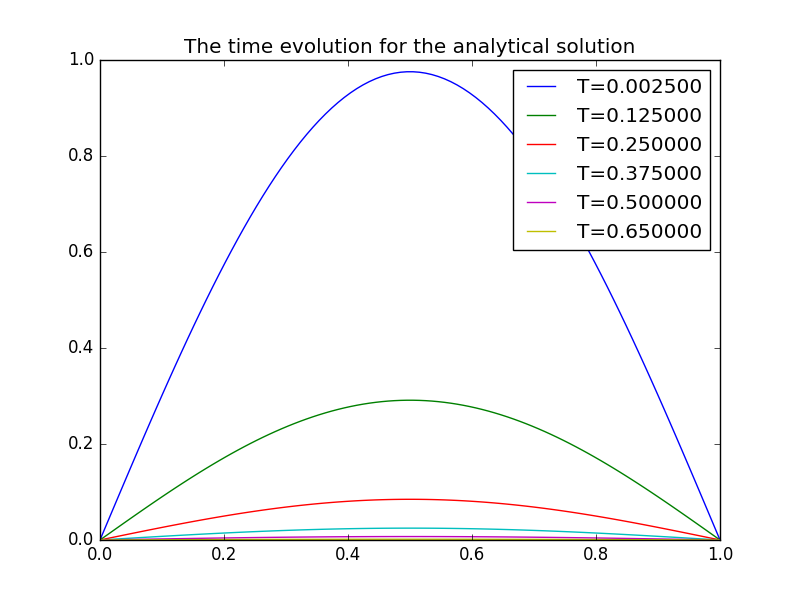
\includegraphics[scale=0.5]{Time_evolution}
    \caption{The time evolution for the analytical solution}
    \label{fig:time_evo}
\end{figure}

\begin{figure}
  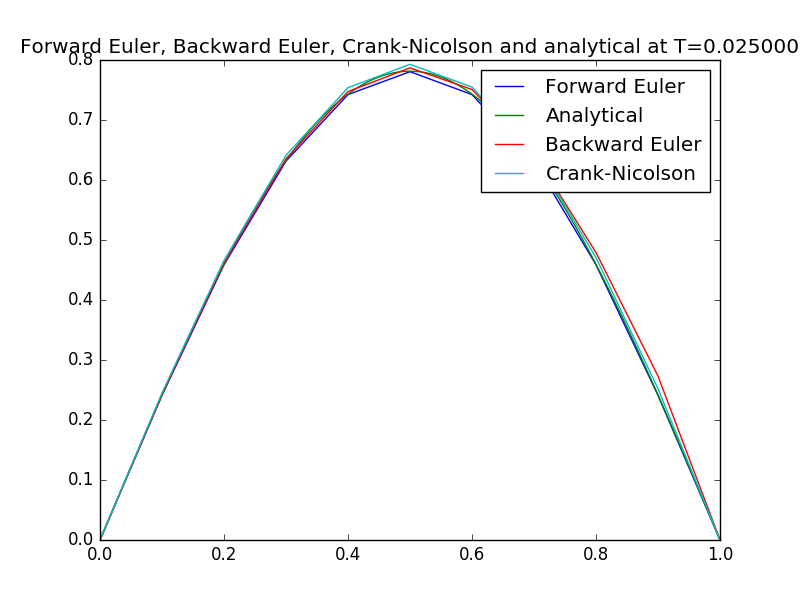
\includegraphics[scale=0.5]{numerical_analytcal_T0025}
    \caption{The three schemes with the analytical solutiion for when $T = 0.025$ and $dt = 0.0025$}
    \label{fig:NumAna0025}
\end{figure}

\begin{figure}
  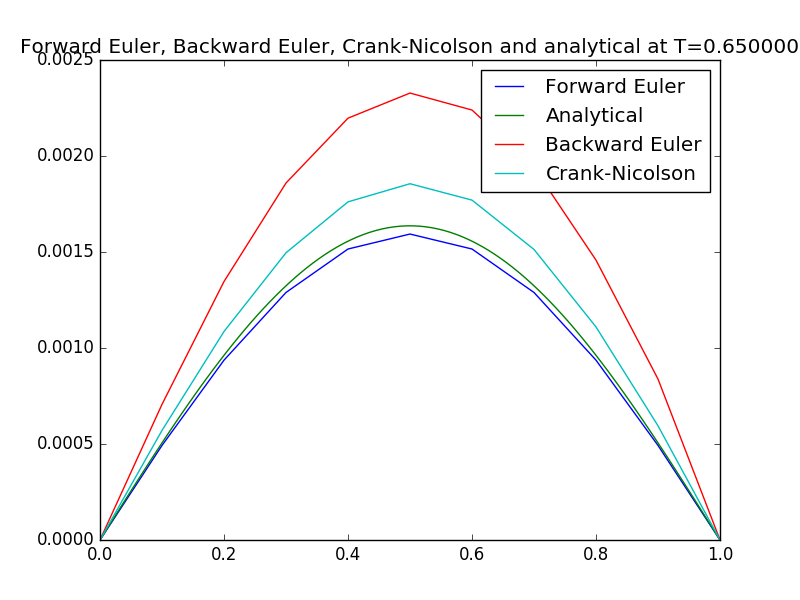
\includegraphics[scale=0.5]{numerical_analytcal_T065}
    \caption{The three schemes with the analytical solutiion for when $T = 0.025$ and $dt = 0.65$}
    \label{fig:NumAna065}
\end{figure}

In figure (\ref{fig:time_evo}) we see the time evolution for the analytical solution which we used to get the time points to analyze the numerical 
calculations.
In figure (\ref{fig:NumAna0025}) and (\ref{fig:NumAna065}) we see the numerical calculations against the analytical for two times $t_1 = 0.025$
and $t_2 = 0.65$. And in table (\ref{tab:RelError}) we see the realtive error at the different time points. Where the relative error is
calculated with the max value and $\epsilon = |1-u_{num}/u_{anałytical}|$.


\begin{table}
\centering
\caption{Table with the relative error of the different schemes calculating it by using the max value and $\epsilon =|1-u_{num}/u_{anałytical}|$ }
\label{tab:RelError}
\begin{tabular}{|l|l|l|}
\hline
 & $t_1=0.025$ & $t_2=0.065$ \\ \hline
Forward Euler & $0.000023$ & $0.026$ \\ \hline
Backward Euler & $0.000631$ & $0.4227$ \\ \hline
Crank Nicolson & $0.01261$  & $0.1341$ \\ \hline
\end{tabular}
\end{table}


\subsection{2D PDE}

\section{Discussion}

\section{Conclusion}

\end{document}
